\documentclass[10pt,a4paper]{article}
\usepackage[margin=2.2cm]{geometry}
\usepackage{fontspec}
\usepackage{kotex}
\setmainfont{Apple SD Gothic Neo}
\setsansfont{Apple SD Gothic Neo}
\usepackage{amsmath,amssymb}
\usepackage{graphicx}
\usepackage{booktabs}
\usepackage{caption}
\usepackage[dvipsnames]{xcolor}
\usepackage[colorlinks=true,linkcolor=MidnightBlue,citecolor=MidnightBlue,
            urlcolor=MidnightBlue]{hyperref}
\usepackage{titlesec}
\titleformat{\section}{\large\bfseries}{\thesection}{0.6em}{}
\titleformat{\subsection}{\normalsize\bfseries}{\thesubsection}{0.5em}{}
\captionsetup{font=small,labelfont=bf}
\setlength{\parskip}{0.35em}
\setlength{\parindent}{0pt}

\usepackage{mdframed}
\newmdenv[linewidth=0.4pt,linecolor=gray!60,backgroundcolor=gray!5,
          innertopmargin=6pt,innerbottommargin=6pt,skipabove=8pt,skipbelow=8pt]{claimbox}
\newcommand{\claim}[2]{\begin{claimbox}\textbf{주장.} #1\par\smallskip
  \textcolor{gray!70}{\textbf{반증 조건.} #2}\end{claimbox}}

\title{\bfseries 아무 말도 안 하는 쪽이 낫다\\[2pt]
\large 판정선은 넘나드는데 기후값은 못 넘는다}
\author{월드모델 실험실 · 노트 $791 \sim 792$}
\date{2026-08-07}
\begin{document}\maketitle

\section{한 줄}

노트 $691$ 이 능력 자를 재고 T$6$ 판정을 발동시켰다 --- \emph{자릿수 오차
$41.95\%$ 가 $30\%$ 선을 넘었으니 이 판의 예보는 순위 전용이다.} 그런데 그
결론은 \textbf{되돌림 하나}(등백분위)에서 나온 것이었다.

되돌림을 \textbf{넷}으로 늘려 봤다. \textbf{판정선은 넘나든다} ---
$41.95\% \leftrightarrow 18.80\%$. \textbf{같은 판, 같은 자료, 같은 자인데
되돌림만 바꿔 T$6$ 의 선을 하나는 넘고 하나는 안 넘는다.}

그리고 \textbf{진짜 기준선을 세우니 전부 못 넘는다.} \textbf{기후값} --- 학습
라벨 평균을 늘 말하고 구간은 학습 라벨 $10{\sim}90$분위 --- 이 자릿수 오차
$\mathbf{0.1656}$ · 덮음 $\mathbf{0.8448}$ 이다. 가장 좋은 되돌림이
$0.1880$ 으로 \textbf{비긴다.}

\textbf{예보를 절대값으로 얹는 것은 아무 말도 안 하는 것과 같다.} 그리고
구간에서는 \textbf{아무 말도 안 하는 쪽이 낫다}($0.8448$ 대 $0.40$).

\begin{figure}[t]\centering
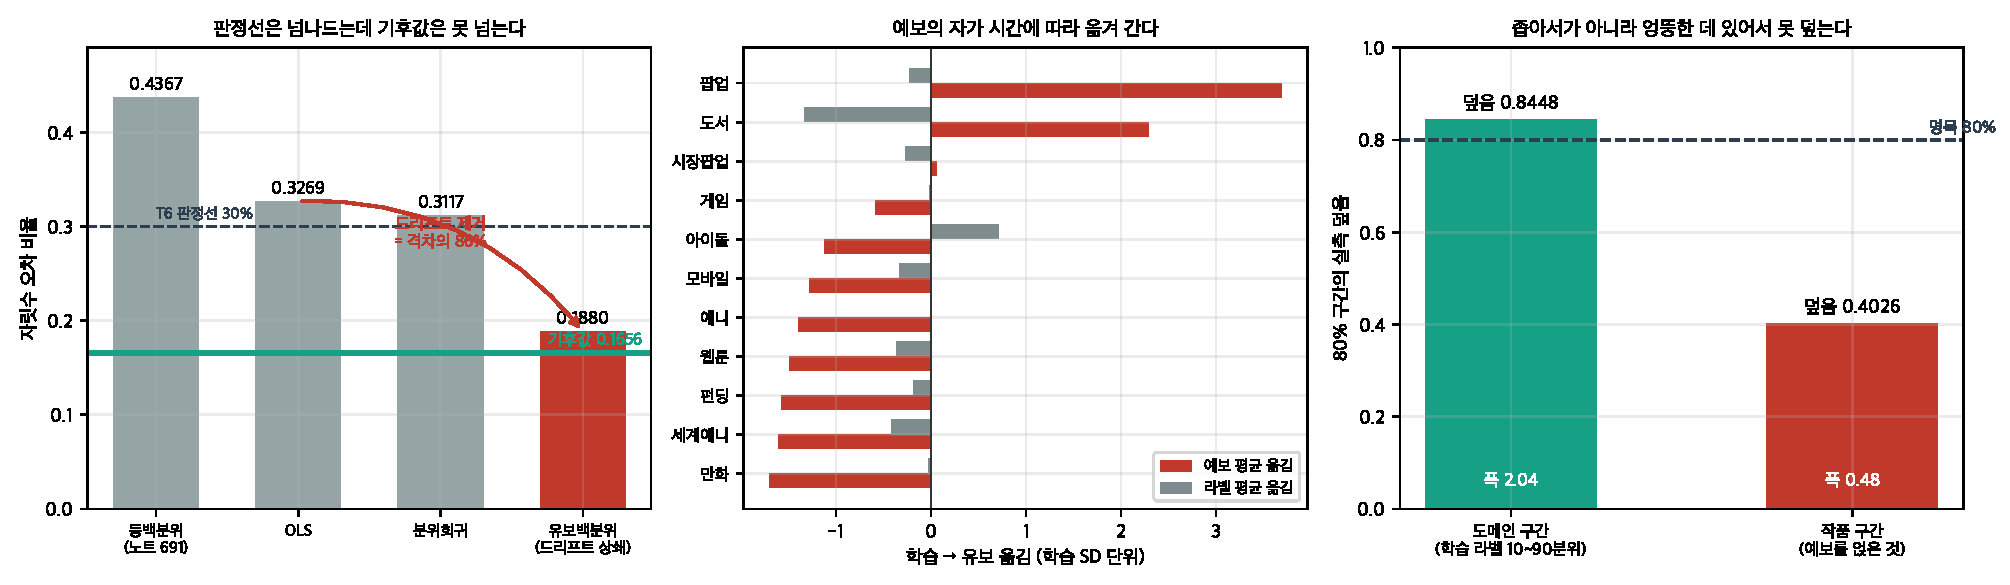
\includegraphics[width=0.99\textwidth]{figs/clim.pdf}
\caption{왼쪽: \textbf{되돌림 넷} --- 점선(T$6$ 판정선)은 넘나들고 초록선(기후값)은
안 넘긴다. 가운데: \textbf{예보의 자가 옮겨 간다} --- 라벨은 안 옮긴다.
오른쪽: \textbf{도메인 구간은 이름값을 하고 작품 구간은 아니다.}}
\end{figure}

\section{먼저 --- 재는 코드가 또 없었다}

노트 $789$ 가 \textbf{규약 $41$}(\emph{법칙을 재는 코드는 저장소에 둔다})을 세운
게 한 사이클 전이다. \textbf{능력 자도 같은 상태였다} --- \texttt{serve/capability.py}
는 \textbf{결론만} 담고 노트 $691$ 의 재는 코드는 스크래치패드와 함께 사라졌다.
그래서 이번엔 \texttt{lab/calib.py} 를 저장소에 만들고 거기서 쟀다.

\textbf{그리고 다시 만들면서 노트 $691$ 의 전제가 틀린 것을 찾았다.} $691$ 은
\emph{``예보는 도메인 안 백분위 꼴(SD $0.126$)''}이라 적었는데, 챔피언
\texttt{F18\_bagboost} 는 그렇지 않다 --- 만화 $8.19 \sim 5{,}621.27$ · 팝업
$1.56 \sim 22.62$ 이고 \textbf{예보 SD 가 도메인마다 $5.6 \sim 1{,}581$ 로
$300$배} 다르다.

\subsection*{그 자에서 내 분위회귀가 발산했다}

첫 실행에서 분위회귀가 자릿수 오차 $\mathbf{0.998}$ 을 냈다 --- 거의 전부 틀린다는
말이라 명백히 고장이다. 고정 학습률이 SD $1{,}581$ 인 자에서 안 먹은 것이다.

\claim{\textbf{내 검증이 너무 쉬웠다.} 손으로 쓴 분위회귀를 \textbf{x SD $=1$
에서만} 시험하고 통과시켰다(덮는 몫 $0.100 \cdot 0.500 \cdot 0.900$ 정확).
\textbf{자가 $300$배 다른 데 쓸 자를 SD $1$ 에서만 검증하면 안 된다.} 표준화해서
풀도록 고치고 x SD $1 \cdot 700 \cdot 0.01$ 세 자에서 다시 확인했다.}
{\textbf{그래도 고장이 눈에 띈 것은 운이 좋았다} --- $0.998$ 은 말이 안 되니까
보였다. \textbf{$0.35$ 쯤 나왔으면 그대로 실었을 것이다.} 이 논문의 다른 숫자
중에 그런 것이 없다는 보장은 없다.}

\section{되돌림 넷과 위약}

\begin{center}
\begin{tabular}{lrrrr}
\toprule
되돌림 & 자릿수 오차 진짜 & 위약 & 덮음 진짜 & 위약 \\
\midrule
등백분위(노트 $691$) & $0.4367$ & $0.4458$ & $0.4122$ & $\mathbf{0.8310}$ \\
OLS & $0.3269$ & $\mathbf{0.1696}$ & $0.3730$ & $\mathbf{0.8347}$ \\
분위회귀 & $0.3117$ & $\mathbf{0.1715}$ & $0.4026$ & $\mathbf{0.8294}$ \\
\bottomrule
\end{tabular}
\end{center}

\textbf{위약이 이긴다} --- 전부 씨앗 SD $3$배 밖이다. 사전등록한 판정 셋이
\emph{(가)} 되돌림이 문제였다 \emph{(나)} 셋 다 위약과 붙는다 \emph{(다)} 구간만
갈린다 였는데 \textbf{어느 것도 발동하지 않았다.}

\claim{\textbf{내 규칙 셋이 전부 ``진짜 $\geq$ 위약''을 전제했다.} \textbf{위약이
이기는 경우를 안 적었다} --- 노트 $770$ 에서 같은 종류의 구멍을 냈고 두 번째다.}
{규칙에 구멍이 있어도 \emph{측정}은 멀쩡하다. \textbf{다만 구멍 난 규칙은 결과를
보고 메우게 되고 그것이 곧 사후 판정이다} --- 이번엔 메우는 대신 \textbf{넷째
결과를 그대로 적고} 다음 사전등록에서 양방향을 다 적었다.}

\subsection*{그 위약이 무엇인지 확인했다 --- 기후값이다}

OLS 위약의 \textbf{기울기가 $10^{-6} \sim 4{\times}10^{-2}$} 이고 \textbf{예측 SD
가 $0.0005 \sim 0.17$} 이다. 즉 위약은 정확히 \textbf{``학습 라벨 평균을 늘 말하는
상수''}이고 구간은 \textbf{학습 라벨 $10{\sim}90$분위}다.

\claim{\textbf{노트 $691$ 의 위약은 약한 상대였다.} 등백분위에서 섞은 예보는
\emph{라벨 분포에서 무작위로 뽑는 것}이라 기후값보다 훨씬 나쁘다. \textbf{그 약한
상대와 비겨서 ``구분 안 된다''로 적혔다.} 같은 위약이 OLS 에서는 기울기 $\approx 0$
으로 무너져 \textbf{기후값이 된다} --- \textbf{위약의 세기가 되돌림에 따라 변한다.}
그래서 위약이 아니라 \textbf{이름 붙이고 값을 못박은 기준선}이 필요하다
(\textbf{규약 $43$}).}
{기후값도 하나의 선택이다 --- \textbf{학습 평균이 아니라 학습 중앙값}을 쓰면
자릿수 오차가 달라진다. \textbf{다만 그것은 결과를 보기 전에 정할 수 있는
선택이고, 섞은 위약은 그렇지 않다.}}

\section{원인 --- 예보의 자가 시간에 따라 옮겨 간다}

\begin{center}
\begin{tabular}{lrrr}
\toprule
& 예보 평균 옮김 & 라벨 평균 옮김 & 되돌린 중심 오차 \\
& (학습 SD 단위) & (학습 SD 단위) & (log$10$) \\
\midrule
팝업 & $\mathbf{+3.69}$ & $-0.23$ & $+0.963$ \\
도서 & $+2.29$ & $-1.33$ & $+0.832$ \\
만화 & $\mathbf{-1.70}$ & $-0.03$ & $-0.824$ \\
세계애니 & $-1.60$ & $-0.42$ & $-0.283$ \\
아이돌 & $-1.12$ & $+0.71$ & $\mathbf{-1.473}$ \\
\bottomrule
\end{tabular}
\end{center}

\textbf{예보는 $-1.7 \sim +3.7$ SD 옮겨 가는데 라벨은 거의 안 옮긴다}(만화 $-0.03$ ·
애니 $+0.00$ · 게임 $-0.02$). 학습에서 맞춘 되돌림 선을 유보 예보에 먹이면
\textbf{중심이 통째로 어긋난다} --- 최대 $1.47$ log$10$, 즉 \textbf{$30$배}.

\claim{\textbf{이것이 노트 $691$ 이 못 준 기제다.} $691$ 은 \emph{``순위 정보가
절대값으로 번역이 안 된다''}로 적었고 \textbf{왜인지는 몰랐다.} \textbf{스피어만은
유보 안에서만 계산되므로 드리프트에 면역이고, 절대값 되돌림은 학습 자에 묶여 있어
면역이 아니다.} 판 $\rho$ $0.4689$ 가 멀쩡한 채로 절대값이 무너지는 이유가 이것이다.}
{드리프트가 \emph{정식화의} 성질인지 \emph{자료의} 성질인지 안 갈랐다 --- 유보에
새 도메인 조합이나 다른 축 덮음이 들어오면 예보 자가 움직일 수 있다.
\textbf{다른 정식화로 같은 드리프트가 나오나 안 쟀다.}}

\subsection*{만화가 결정적 사례다}

만화의 \textbf{진짜 구간이 기후값 구간보다 좁다}($1.109$ 대 $1.484$). 그런데
덮음이 $\mathbf{0.012}$ 대 $\mathbf{0.992}$ 다. \textbf{좁아서 못 덮는 게 아니라
엉뚱한 데 있어서 못 덮는다.}

\section{드리프트를 없애면 --- $86\%$ 가 닫히고 거기서 멈춘다}

유보 예보의 순위를 \textbf{유보 안에서} 매기면 드리프트가 상쇄된다(라벨 쪽은 학습만
본다). \textbf{전이적이라 배치 채점에만 쓸 수 있고 그 한계를 결과 보기 전에 적었다.}

\begin{center}
\begin{tabular}{lrl}
\toprule
OLS(학습 자에 묶임) & $0.3269$ & \\
\textbf{유보 안 백분위}(드리프트 상쇄) & $\mathbf{0.1880}$ & \\
\textbf{기후값} & $\mathbf{0.1656}$ & \\
\midrule
차 & $+0.0224$ & \textcolor{BrickRed}{씨앗 SD $3$배 $0.0275$ \textbf{안} --- \textbf{비긴다}} \\
\bottomrule
\end{tabular}
\end{center}

\textbf{총 격차 $0.1613$ 중 $0.1389$($\mathbf{86.1\%}$)를 드리프트 제거가 닫았다.}
\textbf{남은 $0.0224$ 가 정보 부족이고 그것은 기후값과 구분이 안 된다.}

\claim{\textbf{그래서 T$6$ 판정선 $30\%$ 는 근거가 못 된다.} 되돌림에 따라
$41.95\% \leftrightarrow 18.80\%$ 로 움직이고 \textbf{선을 하나는 넘고 하나는 안
넘는데 둘 다 기후값과 비긴다.} \textbf{절대 자는 이름 붙인 기준선 없이 읽으면
판정이 뒤집힌다} --- 규약 $43$.}
{도메인 $\mathbf{4/11}$ 에서는 기후값을 이긴다 --- 게임 $0.547$ 대 $0.644$ · 아이돌
$0.363$ 대 $0.510$ · 도서 $0.175$ 대 $0.209$ · 애니 $0.136$ 대 $0.150$.
\textbf{전부 라벨이 넓은 도메인이다.} \textbf{그러나 그 넷은 결과를 보고 고른
것이라 그대로 쓰면 체리피킹이다} --- 다음 사전등록에서 \textbf{IQR 문턱을 값으로
먼저 정하고} 갈라야 한다.}

\section{그래도 하나는 팔 수 있다}

\begin{center}
\textbf{도메인 구간}(그 도메인 학습 라벨의 $10{\sim}90$분위)은 덮음
$\mathbf{0.8448}$ 로 \textbf{이름값을 한다.}\\
\textbf{작품 구간}(예보를 얹은 것)은 $\mathbf{0.40}$ 으로 무너진다.
\end{center}

\texttt{serve/capability.py} 를 고쳤다 --- \textbf{``그 도메인의 $80\%$ 구간''을
허용 꼴로 올리고}, \textbf{``그 작품의 $80\%$ 구간''을 금지에 남기고},
자기 검사 문구가 둘을 이름으로 가르게 했다($12/12$ 통과).

\claim{\textbf{T$6$ 이 처음으로 팔 수 있는 것을 하나 늘렸다.} 노트 $691$ 이후
이 트랙은 금지만 늘려 왔다. \textbf{``이 도메인의 팝업은 $80\%$ 가 $300{\sim}8{,}000$명
사이입니다''는 정직한 문장이다} --- 실측이 뒷받침한다.}
{\textbf{그리고 그 문장은 작품에 따라 안 움직인다.} 쓸모가 작다는 뜻이고,
\textbf{예보를 얹는 순간 거짓이 된다.} 파는 쪽에서 그 경계를 지킬 수 있나가
남은 물음이고 그건 측정이 아니라 규율의 문제다.}

\subsection*{그리고 IQR 가설이 맞았다}

노트 $691$ 의 예측 ②(\emph{자릿수 오차가 라벨 \textbf{자리폭}과 정렬한다})가 틀린 뒤
그 자료를 보고 만든 가설이다 --- \emph{자리폭이 아니라 \textbf{집중도}(IQR)다.}

\begin{center}
자릿수 오차와의 스피어만: \textbf{IQR $0.727 \sim 0.909$} 대 자리폭 $0.145 \sim 0.409$
(되돌림 셋 전부)
\end{center}

\claim{\textbf{사후 가설이라 같은 자료로는 판정 못 한다고 먼저 적었고, 기제가 내는
독립 예측을 대신 걸었다} --- \emph{자릿수 오차가 라벨 분포의 자라면 위약의 자릿수
오차도 IQR 과 똑같이 정렬해야 한다.} \textbf{$2/3$ 통과}(등백분위 $0.909/0.927$ ·
분위회귀 $0.845/0.909$ · OLS $0.727/0.900$ 은 차 $0.173$ 로 미달).}
{$2/3$ 는 통과 기준을 내가 $0.15$ 로 정한 결과다. \textbf{도메인이 $11$개라
스피어만의 표준오차가 크고}($n{=}11$ 에서 $\rho\,0.73$ 과 $0.90$ 은 잘 안 갈린다),
\textbf{이 시험은 약하다.}}

\end{document}
